\section{Results and interpretation}
\label{sect:stat}
In this analysis, we examine the data in three different channels and 4 signal regions.
We eventually combine all four bins to utilize more information from the observed and the predicted distributions.
%It was checked that applying the cuts of each channel on other channels do not remain any event and 
%there is not any overlap between the channels, so the channels can be statistically combined.

Backgrounds are taken into account in different categories, including MC Driven, Fake and QCD which are data driven.
%However, due to the method of background estimation in the \tauTau channel \binone,  this channel has one more category 
%called W-jets (W).
As a summary of results, the data and background yields and systematic uncertainties are listed in Table \ref{tbl:yieldSysSummary}. 
\begin{table}[h]
\begin{center}
%\begin{tiny}
\begin{tabular}{c|c|c|c|c}
\hline
\hline
		& \tauTau\binone & \tauTau\bintwo & \eTau\binone & \muTau\binone \\
\hline
MC Driven& 0.75 $\pm$ 0.08 $\pm$ 0.19 & 1.99 $\pm$ 0.87 $\pm$ 0.49  & 0.2 $\pm$ 0.1 $\pm$ 0.05 & 0.45 $\pm$ 0.16  $\pm$ 0.11\\
Fake     &     0.93 $\pm$ 0.32         &           -                 &     2.32 $\pm$ 0.56 $\pm$  0.95 & 1.03 $\pm$ 0.44 $\pm$ 0.44\\
QCD     &     0.15 $\pm$ 0.26         &         0.82 $\pm$ 0.65     &           -              &            -       \\
\hline
SM Total  & 1.83 $\pm$ 0.08 $\pm$ 0.45 & 2.81  $\pm$ 0.87 $\pm$0.81  & 2.55 $\pm$ 0.58 $\pm$ 0.95 & 1.48 $\pm$ 0.47  $\pm$ 0.45\\
\hline
\hline
Observed   & 1     & 2     & 3   & 5 \\  
\hline
%\hline				
%MCD (sta.) & 81x0.00926 &  4x0.39 & 800x0.00025 & 8x0.0563 \\
%\hline
%\multirow{3}{*}{Systematics}&MCD  & 25\%   &   25\% & 25\% & 25\% \\
%                            &DD   & 170\%  &   79\% & 50\% & 69\% \\
%                            &W    & 21\%   &    -  &   -  & - \\
%\hline
\hline
\end{tabular}
\caption{Summary of data and background yields and background uncertainties.}
\label{tbl:yieldSysSummary}
%\end{tiny}
\end{center}
\end{table}
The last row of the table shows the observed data for  each individual channel.  The uncertainties are systematic, unless when there are 
two parts, the first part is statistics.

Since no excess of data over the background prediction is observed, 
we close our study with setting upper limits on the testing signals.
Figure \ref{fig:limit_final}. 
%%%%%%%%%%
\begin{linenomath}
\begin{figure}[h]
\centering
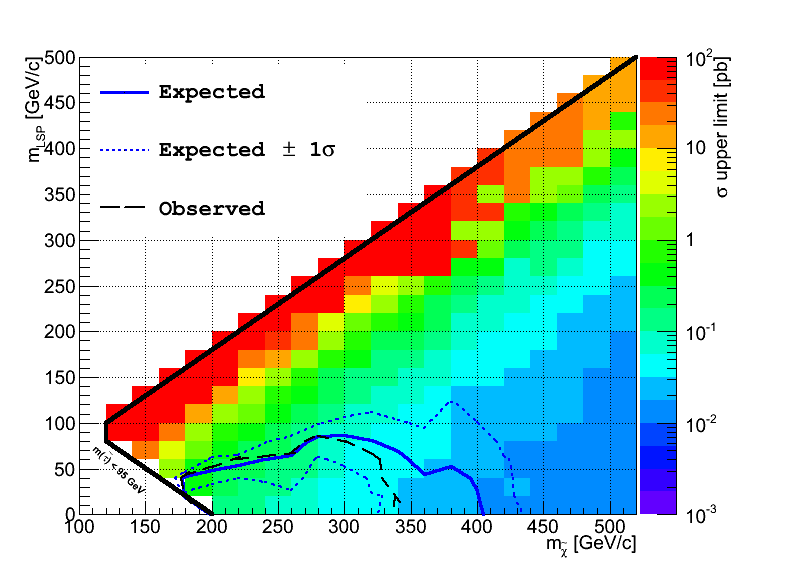
\includegraphics[width=0.7\textwidth,keepaspectratio=true]{StatisticsFig/Exclusion4Bins.png}
\caption{Expected exclusion power in terms of Simplified Models
with the total dataset of 2012. 
%Backgrounds are predicted using Monte-Carlo simulations and a rough estimate of systematic uncertainties equal $10\%$ is taken into account.
}
\label{fig:limit_final}
\end{figure}
\end{linenomath}
%%%%%%%%%%
shows the expected and observed upper limit on the cross section of the chargino pair production in terms of Simplified Models.% \cite{Alwall:2008ag,alves:sms}. 
It is shown that the analysis rules out the \chione up to XXX \GeV and  $\PSGczDo$ = YYY \GeV.

